\documentclass[12pt]{beamer}
\usepackage[utf8]{inputenc}
\usepackage[spanish]{babel}
\usepackage{graphicx}
\usepackage{amsmath}
\usepackage{amsfonts}
\usepackage{amssymb}
\usepackage{amsthm}
\usepackage{listings}
\usetheme{Madrid}
%\usetheme{JuanLesPins}
%\usetheme{Montpellier}
%\usetheme{Berkeley}
%\usetheme{PaloAlto}
\usefonttheme{serif}
\usepackage{verbatim}
\usepackage{booktabs}

\title{Curso de \LaTeX}
%\author{Nombre del Autor}
\date{\today}

\begin{document}
\begin{frame}
\titlepage
\end{frame}
%%%%%%
\begin{frame}
\tableofcontents
\end{frame}
%%%%%%
\section{Introducción}
\begin{frame}{¿Qué es \LaTeX?}
  \begin{itemize}
    \item \LaTeX{} es un sistema de preparación de documentos.
    \item<2-> Utilizado para la creación de documentos científicos y técnicos.
  \end{itemize}
\end{frame}
%%%%%%
\begin{frame}{¿Qué se necesita?}
  \begin{itemize}
    \item A diferencia de muchos programas informáticos, \LaTeX{} no es una única aplicación que lo ``contenga todo'' en un solo lugar.
    \item<2-> En cambio, consta de programas separados que trabajan en conjunto.
    \item<3-> Podemos dividirlos en dos elementos que realmente se necesitan:
    \begin{itemize}
      \item<4-> Un sistema TeX.
      \item<5-> Un editor de texto.
    \end{itemize}
  \end{itemize}  
\end{frame}
%%%%%%
\begin{frame}{Sistema \LaTeX}
  \begin{itemize}
    \item<1-> El núcleo del trabajo con \LaTeX{} es tener disponible un sistema TeX. 
    \item<2-> Un sistema TeX es un conjunto de programas y archivos necesarios para que \LaTeX{} funcione.
    \item<3-> Existen dos sistemas TeX principales: MiKTeX y TeX Live. Ambos disponibles para Windows, macOS y Linux.
    \item<4-> MiKTeX tiene un fuerte respaldo en Windows; en macOS, TeX Live está incluido en una colección más grande llamada MacTeX.
  \end{itemize}
\end{frame}
%%%%%%
\begin{frame}{Editor de Texto}
  \begin{itemize}
    \item Los archivos de \LaTeX{} son archivos de texto plano con extensión {\color{blue}\texttt{.tex}}, por lo que pueden editarse con cualquier editor de texto.
    \item<2-> Sin embargo, es conveniente utilizar un editor diseñado para trabajar con LaTeX, ya que ofrecen funciones como:
    \begin{itemize}
      \item<3-> Compilación de archivos con un solo clic.
      \item<4-> Visores de PDF integrados.
      \item<5-> Resaltado de sintaxis.
    \end{itemize}
    \item<6-> Existen muchos editores de \LaTeX{}, entre los que podemos enumerar.
    \begin{itemize}
      \item<7-> TeXworks, está incluido en TeX Live y MiKTeX para Windows y Linux
      \item<8-> TeXShop, incluido en MacTeX.
      \item<9-> Winedt, un editor comercial para Windows.
      \item<10-> Overleaf, un editor en línea.
    \end{itemize}    
  \end{itemize}
\end{frame}
%%%%%%
\begin{frame}{Editor de Texto}  
    \begin{figure}
      \centering
      
\includegraphics[width=0.8\textwidth]{Editores.png}
      \caption{Distintos editores de \LaTeX.}
      \label{fig:ejemplo_imagen}
    \end{figure}
\end{frame}
%%%%%%
\section{Estructura Básica}
\subsection{Documento Mínimo}
\begin{frame}{Documento Mínimo}
  \begin{itemize}
    \item La estructura básica de un documento es la siguiente:
    \begin{center}
    \begin{minipage}{0.5\textwidth}          
    \begin{block}{}       
       \color{blue}
        \texttt{\textbackslash documentclass\{article\}\\
        \textbackslash begin\{document\}\\
         \hspace{1cm}Hello World!\\
        \textbackslash end\{document\}}
      \end{block}
      \end{minipage}
    \end{center}
    \item<2-> El comando {\color{blue}\texttt{\textbackslash documentclass}} indica el tipo de documento que se va a crear.
    \item<3-> El \emph{argumento} en llaves {\color{blue}\texttt{\{} \texttt{\}}} le dice a \LaTeX{} qué tipo de documento estamos creando: en este ejemplo, {\color{blue}\texttt{article}}.
    \item<4-> Un signo de porcentaje {\color{blue}\texttt{\%}} comienza un \emph{comentario} --- \LaTeX{} ignorará el resto de la línea.
  \end{itemize}
\end{frame}
%%%%%%
\begin{frame}{\texttt{\textbackslash documentclass}}
  \begin{itemize}
    \item {\color{blue}\texttt{\textbackslash documentclass}} es un comando que le dice a \LaTeX{} qué tipo de documento estamos creando.
    \item<2-> Algunos tipos de documentos comunes son:
    \begin{itemize}
      \item {\color{blue}\texttt{article}}: Artículos de revistas, presentaciones, informes cortos, documentación, invitaciones, etc.
      \item<3-> {\color{blue}\texttt{report}}: Informes más largos que contienen varios capítulos, libros pequeños, tesis, etc.
      \item<4-> {\color{blue}\texttt{book}}: Libros.
      \item<5-> {\color{blue}\texttt{letter}}: Cartas.
      \item<6-> {\color{blue}\texttt{beamer}}: Presentaciones.
    \end{itemize}
  \end{itemize}
\end{frame}
%%%%%%
\begin{frame}{\texttt{\textbackslash documentclass}}
  \begin{itemize}
    \item<1-> El comando {\color{blue}\texttt{\textbackslash documentclass}} posee conjuntos de opciones que van entre corchetes {\color{blue}\texttt{[ ]}}. Algunas de ellas son:
    \begin{itemize}
      \item {\color{blue}\texttt{10pt, 11pt, 12pt}}: Tamaño de la fuente.
      \item<2-> {\color{blue}\texttt{a4paper, letterpaper, legalpaper}}: Tamaño del papel.
      \item<3-> {\color{blue}\texttt{twocolumn}}: Dos columnas.
      \item<4-> {\color{blue}\texttt{twoside, oneside}}: Impresión a doble o una cara.
    \end{itemize}
    \item<5-> Por ejemplo, {\color{blue}\texttt{\textbackslash documentclass[12pt,a4paper]\{article\}}} indica que el documento será un artículo con fuente
    de 12 puntos y tamaño de papel A4.
  \end{itemize}
\end{frame}
%%%%%%
\subsection{Paquetes}
\begin{frame}{Paquetes}
  \begin{itemize}
    \item<1->Los paquetes son archivos que contienen comandos y entornos adicionales para \LaTeX.
    \item<2-> Se cargan en el preámbulo del documento después del comando {\color{blue}\texttt{\textbackslash documentclass}}.
    \item<3-> El comando {\color{blue}\texttt{\textbackslash usepackage[]\{\}}} permite cargar un complemento (plugin), que añade nuevas funcionalidades.
    \end{itemize}    
\end{frame}  
%%%%%%
\begin{frame}{Paquetes}
  \begin{itemize}
    \item<1-> Existen numerosos complementos (por ejemplo, para mostrar imágenes, crear tablas, dibujar fórmulas químicas, generar cuadrículas de sudoku, etc.).

    {\color{red} Ejemplos}:
    \begin{itemize}
      \item<2-> {\color{blue}\texttt{\textbackslash usepackage[utf8]\{inputenc\}}}: Carga el paquete inputenc con la opción utf8 (esto es para la codificación de caracteres).
      \item<3-> {\color{blue}\texttt{\textbackslash usepackage[T1]\{fontenc\}}}: Especifica que se está utilizando el paquete de fuentes T1.
      \item<4-> {\color{blue}\texttt{\textbackslash usepackage[spanish]\{babel\}}}: Carga el paquete babel, que se encarga de la tipografía con el idioma español.
      \item<5-> {\color{blue}\texttt{\textbackslash usepackage\{graphicx\}}}: Carga el paquete que permite incluir imágenes externas en el documento.
    \end{itemize}
  \end{itemize}
\end{frame}
%%%%%%
\subsection{Entornos}
\begin{frame}{Entornos}
  \begin{itemize}
    \item<1-> Los entornos definen un ``bloque'': todo el texto dentro de este bloque se transformará según la función del entorno.
    \item<2-> Un entorno siempre comienza con {\color{blue}\texttt{\textbackslash begin\{\}}} y termina con {\color{blue}\texttt{\textbackslash end\{\}}}. Dentro de las {\color{blue}\{ \}} se especifica el nombre del entorno.
    \item<3-> El entorno {\color{blue}\texttt{document}} es obligatorio: lo que está dentro constituye el contenido del documento. Fuera del bloque document, se encuentran comandos que modifican las características del documento o cómo se imprime (por ejemplo, paquetes o comandos globales).
    \item <4-> Todos los demás entornos son opcionales y se usan según sea necesario.
    
    {\color{red}Ejemplo}:
    El entorno {\color{blue}\texttt{itemize}} crea listas con viñetas (listas sin numerar). Por lo tanto, una lista con viñetas se crea cada vez que se llama al comando {\color{blue}\texttt{\textbackslash item}}.
  \end{itemize}
\end{frame}
%%%%%%
\subsection{Dando Formato al texto}
\begin{frame}{Dando Formato al texto}
  \LaTeX{} tiene comandos para dar formato al texto.
  \begin{itemize}
    \item<1-> {\color{blue}\texttt{\textbackslash textbf\{texto\}}}: \textbf{Texto en negrita}.
    \item <2-> {\color{blue}\texttt{\textbackslash textit\{texto\}}}: \textit{Texto en cursiva}.
    \item <3-> {\color{blue}\texttt{\textbackslash underline\{texto\}}}: \underline{Texto subrayado}.
    \item <4-> {\color{blue}\texttt{\textbackslash texttt\{texto\}}}: \texttt{Texto en fuente de máquina de escribir}.
    \item <5-> {\color{blue}\texttt{\textbackslash color\{nombre color\}}}: \color{green}{Texto en color}.
    \item<6-> Formato de tamaño de fuente: {\color{blue}\texttt{\textbackslash tiny}}, {\color{blue}\texttt{\textbackslash scriptsize}}, {\color{blue}\texttt{\textbackslash footnotesize}}, {\color{blue}\texttt{\textbackslash small}}, {\color{blue}\texttt{\textbackslash normalsize}}, {\color{blue}\texttt{\textbackslash large}}, {\color{blue}\texttt{\textbackslash Large}}, {\color{blue}\texttt{\textbackslash LARGE}}, {\color{blue}\texttt{\textbackslash huge}}, {\color{blue}\texttt{\textbackslash Huge}}.
    \item<7-> Forzar un salto de línea: {\color{blue}\texttt{\textbackslash\textbackslash}}. 
  \end{itemize}
\end{frame}
%%%%%%
\section{Listas}
\begin{frame}{Dando Formato al texto}
  El entorno {\color{blue}\texttt{itemize}} crea listas con viñetas (listas sin numerar).
  \begin{center}
    \begin{minipage}{0.5\textwidth} 
  \begin{block}{}
    \texttt{\textbackslash begin\{itemize\}\\
      \textbackslash item Elemento 1\\
      \textbackslash item Elemento 2\\
      \textbackslash item Elemento 3\\
    \textbackslash end\{itemize\}}
  \end{block}
  \end{minipage}
  \end{center}
  \begin{itemize}
    \item Elemento 1
    \item Elemento 2
    \item Elemento 3
  \end{itemize}
\end{frame}
%%%%%%
\begin{frame}{Dando Formato al texto}
  El entorno {\color{blue}\texttt{enumerate}} crea listas numeradas.
  \begin{center}
    \begin{minipage}{0.5\textwidth} 
  \begin{block}{}
    \texttt{\textbackslash begin\{enumerate\}\\
      \textbackslash item Elemento 1\\
      \textbackslash item Elemento 2\\
      \textbackslash item Elemento 3\\
    \textbackslash end\{enumerate\}}
  \end{block}
  \end{minipage}
  \end{center}
  \begin{enumerate}
    \item Elemento 1
    \item Elemento 2
    \item Elemento 3
  \end{enumerate}
\end{frame}
%%%%%%
\section{Secciones}
\begin{frame}{Secciones}
  LaTeX puede dividir/estructurar documentos en múltiples niveles jerárquicos, dependiendo del tipo de documento con el que se trabaje.
  \begin{itemize}
    \item<1-> {\color{blue}\texttt{\textbackslash section\{texto\}}}: Secci\'on.
    \item<2-> {\color{blue}\texttt{\textbackslash subsection\{texto\}}}: Subsecci\'on.
    \item<3-> {\color{blue}\texttt{\textbackslash subsubsection\{texto\}}}: Subsubsecci\'on.
    \item <4-> {\color{blue}\texttt{\textbackslash paragraph\{texto\}}}: Párrafo.
    \item <5-> {\color{blue}\texttt{\textbackslash subparagraph\{texto\}}}: Subpárrafo.
    \item <6-> {\color{blue}\texttt{\textbackslash chapter\{texto\}}}: Cap\'itulo.
  \end{itemize}
\end{frame}
%%%%%%
\begin{frame}{Secciones}
  \begin{center}
    \begin{minipage}{0.8\textwidth}
  \begin{block}{}
    \footnotesize
    \textbackslash documentclass\{article\}\\
    \textbackslash usepackage[T1]\{fontenc\}\\
    \textbackslash begin\{document\}\\
\hspace{1cm}Hola Mundo!\\[10pt]
\hspace{1cm}Primer Documento.\\[10pt]

\hspace{1cm}\textbackslash section\{Primera Sección\}\\
\hspace{1cm}Texto de la primera sección.\\[10pt]

\hspace{1cm}Segundo Párrafo.\\[10pt]

\hspace{1cm}\textbackslash subsection\{Subseccion de la primera sección\}\\

\hspace{1cm}Texto de la subsección.\\[10pt]

\hspace{1cm}\textbackslash subsubsection\{Subsubsección de la primera sección\}\\

\hspace{1cm}Texto de la subsubsección.\\

\textbackslash end\{document\}\\
  \end{block}
  \end{minipage}
  \end{center}
\end{frame}
%%%%%%
\begin{frame}{Secciones}
  \begin{center}
    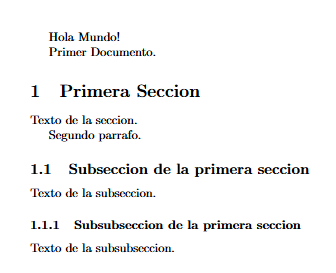
\includegraphics[scale=0.9]{Secciones.png}  
  \end{center}
\end{frame}
%%%%%%
\begin{frame}{Aclaraciones}
  \begin{itemize}
    \item Las comillas son un poco complicadas: use el acento invertido \texttt{\`{}} sobre el lado izquierdo y el apóstrofe \texttt{'{}} sobre el lado derecho.
      
  \begin{tabular}{ll}
     Comillas simple: & `texto'.\\  
   Comillas dobles: & ``texto''.
  \end{tabular}
    \item<2-> Algunos caracteres comunes tienen significados especiales en \LaTeX:  
  \begin{center}
    \begin{tabular}{cl}
      \texttt{\%} & Signo de porcentaje \\
      \texttt{\#} & Signo numeral \\
      \texttt{\&} & Ampersand                 \\
      \texttt{\$} & Signo pesos               \\
    \end{tabular}
  \end{center}
    \item<3-> Si son usados, tendremos errores en la compilación. Para usar estos caracteres en la salida, se debe colocar barra invertida al caracter.
      \begin{center}
      \begin{minipage}{3.5cm}
        \begin{block}{}        
          \textbackslash\$\hspace{10pt}\textbackslash\%\hspace{10pt}\textbackslash\&\hspace{10pt}\textbackslash\#!              
      \end{block}
      \end{minipage}
    \end{center}      
  \end{itemize}  
\end{frame}
%%%%%%
\begin{frame}{Aclaraciones}
  \begin{itemize}
    \item<1-> Los espacios en blanco en el código fuente de \LaTeX{} no tienen ningún efecto en el documento final.
    \item<2-> \LaTeX{} trata los espacios en blanco como ``espacios en blanco''.
    \item<3-> Para obtener un espacio en blanco en el documento final, se deben usar comandos especiales.
    \item<4-> Para obtener un espacio en blanco en el documento final, se deben usar comandos especiales.    
  \end{itemize}
\end{frame}
%%%%%
\begin{frame}{Tipografía Matemática}
   \footnotesize{
     \begin{itemize}
     \item<1-> ¿Por qué son especiales los signos pesos \texttt{\color{blue}\$}? Los usamos para marcar contenido  matemático en el texto.\\[1ex]    
     \begin{tabular}{|p{5cm}|p{5cm}|}\hline
 \color{green}\% no tan bueno: & \\
 Sean a y b tales que c = a - b + 1.&Sean a y b tales que c = a - b + 1.\\
 \color{green}\% mucho mejor: & \\
 Sean \$a\$ y \$b\$ tales que \$c = a - b + 1\$. &
 Sean $a$ y $b$ tales que $c = a - b + 1$.\\\hline
     \end{tabular}
   \item<2-> Utilice siempre los signos de pesos en pares --- uno para comenzar el contenido matemático, y uno para terminarlo.
   \item<3-> \LaTeX{} maneja el espacio automáticamente; por lo que ignorará los que se hayan puesto.\\[1ex]
     \begin{center}    
     \begin{tabular}{|l|l|}\hline
 Sea \$y=mx+b\$ \ldots & Sea $y=mx+b$ \ldots\\[5pt]      
 Sea \$y = m x + b\$ \ldots & Sea $y = m x + b$ \ldots\\\hline
     \end{tabular}
     \end{center}
\end{itemize}
}   
\end{frame}
%%%%%%
\begin{frame}{Tipografía Matemática:Notaci\'on}
  \begin{itemize}
    \item<1-> Use el signo \texttt{\^} para indicar superíndices y el
    guión bajo \texttt{\_} para marcar subíndices.

    \begin{tabular}{|l|l|}\hline
      \texttt{\$y = c\_2 x\texttt{\^}2 + c\_1 x + c\_0\$} & $y = c_2 x^2 + c_1 x + c_0$\\\hline
    \end{tabular}
    \vskip 2ex
    
  \item<2-> Utilice las llaves \texttt{\{} \texttt{\}} para
    agrupar superíndices y subíndices.
    \begin{tabular}{|l|l|}\hline      
\texttt{\$F\_n = F\_n-1 + F\_n-2\$ \% oops!} & $F_n = F_n-1 + F_n-2$\\ 
\texttt{\$F\_n = F\_\{n-1\} + F\_\{n-2\}\$ \% ok!} & $F_n = F_{n-1} + F_{n-2}$\\\hline
    \end{tabular}
    \vskip 2ex
    
  \item<3-> Hay comandos para letras Griegas y notación común.
    \begin{tabular}{|l|l|}\hline
      \texttt{\$\textbackslash mu = A e\^\{Q/RT\}\$} & $\mu = A e^{Q/RT}$\\
      \texttt{\$\textbackslash Omega = \textbackslash sum\_\{k=1\}\texttt{\^}n \textbackslash omega\_k\$} & $\Omega = \sum_{k=1}^{n} \omega_k$\\\hline
    \end{tabular}
  \end{itemize}
\end{frame}
%%%%%%
 \begin{frame}[fragile]{Tipografía Matemática: Entornos}
   \begin{itemize}
   \item {\color{blue}\texttt{equation}} es un \emph{entorno}.
   \item<2-> Un comando puede producir diferentes salidas en diferentes contextos.
   \begin{columns}
     \begin{column}{0.5\textwidth}
       Podemos escribir {\color{blue}
 \texttt{\$\textbackslash Omega = \textbackslash sum\_\{k=1\}\texttt{\^}\{n\} \textbackslash omega\_k\$}}
 en nuestro texto, o podemos escribir{\color{blue}
 \textbackslash begin\{equation\}
   \textbackslash Omega = \textbackslash sum\_\{k=1\}\texttt{\^}\{n\} \textbackslash omega\_k
 \textbackslash end\{equation\}}

 para mostrarlo en un entorno diferente.
     \end{column}
    \begin{column}{0.01\textwidth}
      \vline
    \end{column}
     \begin{column}{0.5\textwidth}
       Podemos escribir
       $ \Omega = \sum_{k=1}^{n} \omega_k$
       en nuestro texto, o podemos escribir
 \begin{equation}
   \Omega = \sum_{k=1}^{n} \omega_k
 \end{equation}
 para mostrarlo en un entorno diferente.
     \end{column}
   \end{columns}    
     \vskip 2ex
   \item<3-> Note como el $\Sigma$ es más grande en el entorno \texttt{equation}, y como el subíndice y superíndice cambian de
     posición, a pesar de que utilizamos los mismos comandos.
   \end{itemize}
 \end{frame}
%%%%%%
\begin{frame}[fragile]{Ejemplos con {\color{green}\texttt{amsmath}}}
  \begin{itemize}
  \item Utilice \texttt{equation*} (``ecuación-asterisco'') para
    ecuaciones no-numeradas.
    \begin{tabular}{ll}
     \begin{minipage}{0.5\textwidth}
      \color{blue}
      \textbackslash begin\{equation*\}\\
      \textbackslash Omega = \textbackslash sum\_\{k=1\}\texttt{\^}\{n\} \textbackslash omega\_k\\
      \textbackslash end\{equation*\}
     \end{minipage} &
     \begin{minipage}{0.4\textwidth}
     \begin{equation*}
     \Omega = \sum_{k=1}^{n} \omega_k
     \end{equation*}
     \end{minipage}
    \end{tabular}
   \item<2-> \LaTeX{} trata las letras adyacentes como variables multiplicadas entre sí, lo cual no siempre es lo que se quiere. \texttt{amsmath} define comandos para muchos operadores matemáticos comunes.
   \begin{tabular}{ll}
    \begin{minipage}{0.6\textwidth}
      \color{red}
        \textbackslash begin\{equation*\} \% bad!\\
        min\_\{x,y\} (1-x)\texttt{\^}2\\
        \textbackslash end\{equation*\}\\
      \color{blue}
        \textbackslash begin\{equation*\} \% good!\\
        \textbackslash min\_\{x,y\}\{(1-x)\texttt{\^}2\}\\
        \textbackslash end \{equation*\} 
    \end{minipage} &
    \begin{minipage}{0.2\textwidth}
        \begin{equation*} % bad!
          min_{x,y} (1-x)^2
        \end{equation*}
      \begin{equation*} % good!
          \min_{x,y}{(1-x)^2}
      \end{equation*}
    \end{minipage}
   \end{tabular}
  \end{itemize}
\end{frame}
%%%%%%
\begin{frame}[fragile]{Ejemplos con \texttt{\color{green}amsmath}}
  \footnotesize{
  \begin{itemize}
    \item<1-> Alinear una secuencia de ecuaciones al signo igual
      \begin{align*}
        (x+1)^3 &= (x+1)(x+1)(x+1) \\
        &= (x+1)(x^2 + 2x + 1) \\
        &= x^3 + 3x^2 + 3x + 1
      \end{align*}
      con el entorno \texttt{align*}.
    \item<2-> El ampersand \texttt{\&} separa la columna izquierda (antes del $=$) de la columna derecha (después del $=$).
    \begin{center}
    \begin{minipage}{0.55\textwidth}
    \begin{block}{}
\texttt{\color{blue}
\textbackslash begin\{align*\}\\
(x+1)\texttt{\^}3 \&= (x+1)(x+1)(x+1) \textbackslash\textbackslash\\
\&= (x+1)(x\texttt{\^}2 + 2x + 1) \textbackslash\textbackslash\\
\&= x\texttt{\^}3 + 3x\texttt{\^}2 + 3x + 1\\
\textbackslash end\{align*\}}  
    \end{block}     
  \end{minipage}  
\end{center}
     \item<3-> Una doble barra invertida
       \texttt{\textbackslash\textbackslash} da comienzo a una nueva línea.     
\end{itemize}}
\end{frame}
%%%%%%
\begin{frame}[fragile]{Etiquetas y Referencias Cruzadas}
  \begin{itemize}
    \item<1-> Utilice {\color{blue}\texttt{label}} y {\color{blue}\texttt{ref}} para la numeración automática.
    \item<2-> El paquete {\color{blue}\texttt{amsmath}} proporciona {\color{blue}\texttt{eqref}} para las referencias de ecuaciones.
    \end{itemize} 
    \uncover<3->{
\begin{tabular}{lc}
  \begin{minipage}{0.35\linewidth}\color{blue} \tiny   
    \textbackslash documentclass\{article\}\\
    \textbackslash usepackage\{amsmath\} \% para \textbackslash eqref\\

    \textbackslash begin\{document\}\\

    \textbackslash section\{Introducti\'on\}\\
    \textbackslash label\{sec:intro\}\\

En la Sección \textbackslash ref\{sec:metodo\},
hemos \ldots\\

\textbackslash section\{M\'etodo\}\\
\textbackslash label\{sec:metodo\}\\

\textbackslash begin\{equation\}\\
\textbackslash label\{eq:euler\}\\
e\texttt{\^}\{i\textbackslash pi\} + 1 = 0\\
\textbackslash end\{equation\}\\

Por \textbackslash eqref\{eq:euler\}, Tenemos \ldots\\

\textbackslash end\{document\}
  \end{minipage} & \begin{minipage}{\textwidth}
    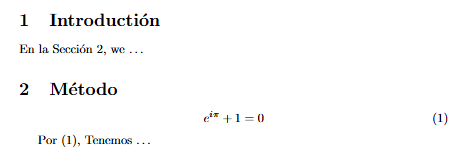
\includegraphics[scale=0.6]{Referencias.png}
  \end{minipage}
   \end{tabular}}
\end{frame}
%%%%%%
\begin{frame}{Usando Im\'agenes}
  \begin{itemize}
    \item Para importar im\'agenes en \LaTeX, se usa el paquete \texttt{\color{blue}graphicx},
     que añade el comando \texttt{\color{blue}includegraphics} a \LaTeX{}.
    \item<2-> El comando \texttt{\color{blue}includegraphics} toma un argumento obligatorio, que es el nombre del archivo de la imagen.
    \item<3-> Se puede insertar ficheros EPS, PNG, JPG y PDF. Si dispone de varias versiones de la imagen entonces se puede escribir la extensión.
  \end{itemize}
  \uncover<4->{
  \begin{tabular}{ll}
    \begin{minipage}{0.5\textwidth}
      \begin{block}{}
        \texttt{\color{blue}
          \textbackslash usepackage\{graphicx\}\\
          \textbackslash begin\{document\}\\
          \textbackslash includegraphics\{imagen.png\}\\
          \textbackslash end\{document\}
        }
      \end{block}
    \end{minipage} &
    \begin{minipage}{0.4\textwidth}
      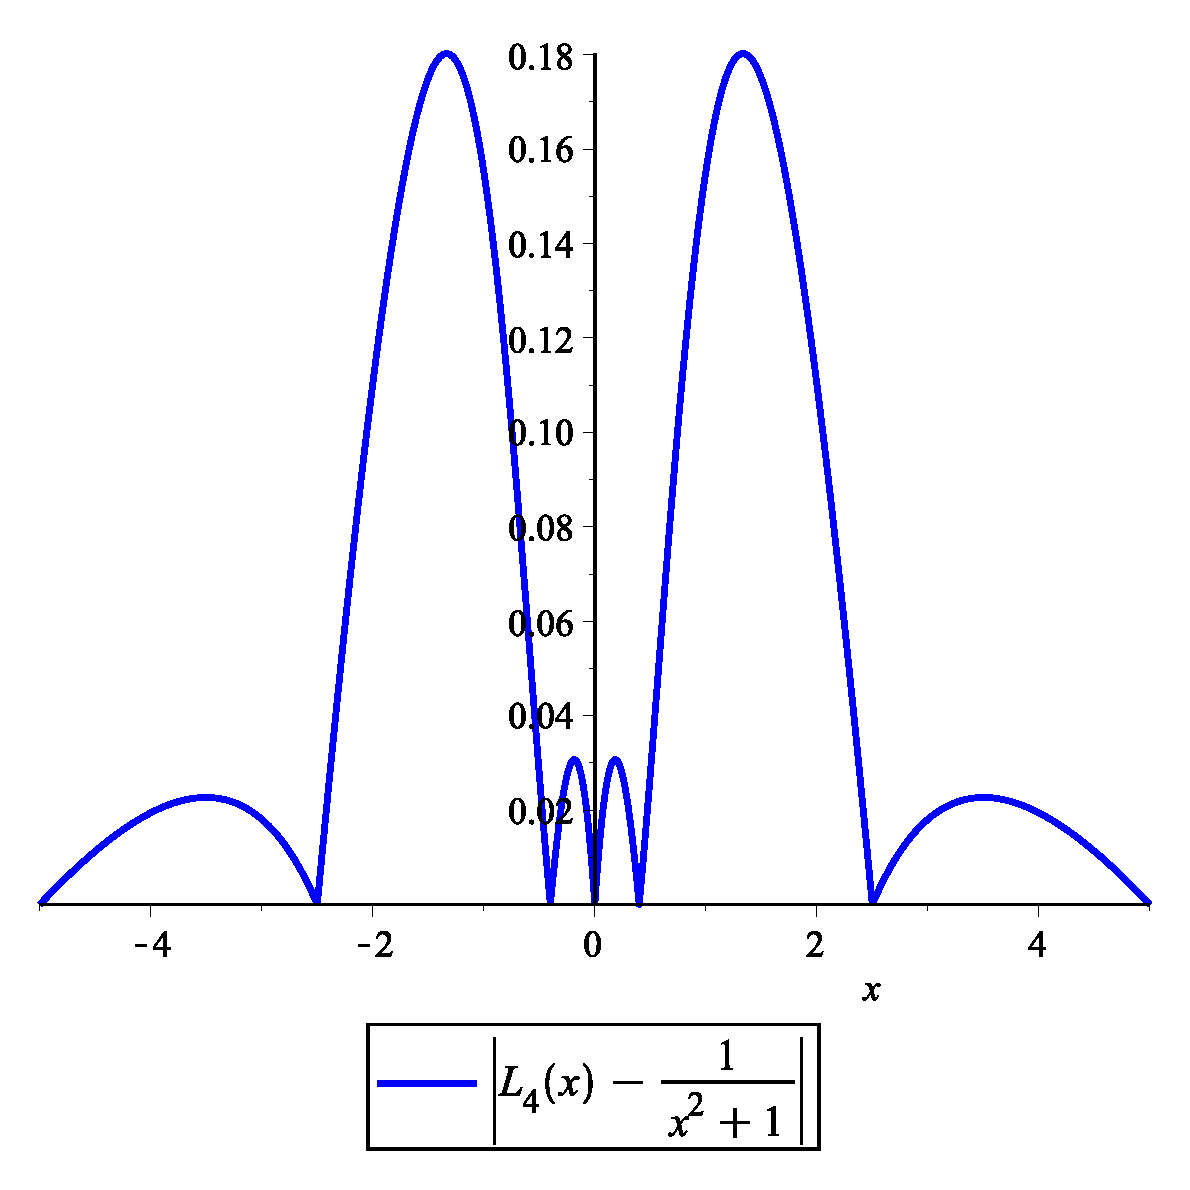
\includegraphics[scale=0.2]{err_L4.eps}
    \end{minipage}
  \end{tabular}}
\end{frame}
%%%%%%
\begin{frame}{Cambiando la apariecia de la imagen}
  \begin{itemize}
    \item El comando \texttt{\color{blue}includegraphics} tiene opciones para cambiar la apariencia de la imagen.
    \item<2-> Opciones para controlar el tamaño y la forma de las imágenes incluidas, pudiendo incluso recortarlas. 
    \item<3-> La opción más sencilla es definir el anchura y alto de una imagen, las cuales se pueden dar de forma relativa con respecto al ancho \texttt{\color{blue}\textbackslash textwidth} y al alto \texttt{\color{blue}\textbackslash textheight} de la zona de texto.
    \item<4-> \LaTeX{} ajustará la escala de la imagen automáticamente para que la proporción de las dimensiones de la imagen sea la correcta.
    \item <5-> Para cambiar el ancho se puede usar \texttt{\color{blue}\textbackslash includegraphics[width=0.5\textbackslash textwidth]\{imagen.png\}}.
    \item <6-> Para cambiar la altura, se puede usar \texttt{\color{blue}\textbackslash includegraphics[height=0.5\textbackslash textheight]\{imagen.png\}}.
  \end{itemize}
\end{frame}
%%%%%%
\begin{frame}{Cambiando la apariecia de la imagen}
  \begin{tabular}{ll}
    \begin{minipage}{0.65\textwidth}
      \scriptsize
      \begin{block}{}
        \texttt{\color{blue}
          \textbackslash usepackage\{graphicx\}\\
          \textbackslash begin\{document\}\\
          \textbackslash includegraphics[width=0.25\textbackslash textwidth]\{imagen.png\}\\
          \textbackslash end\{document\}
        }
      \end{block}
    \end{minipage} &
    \begin{minipage}{0.4\textwidth}
      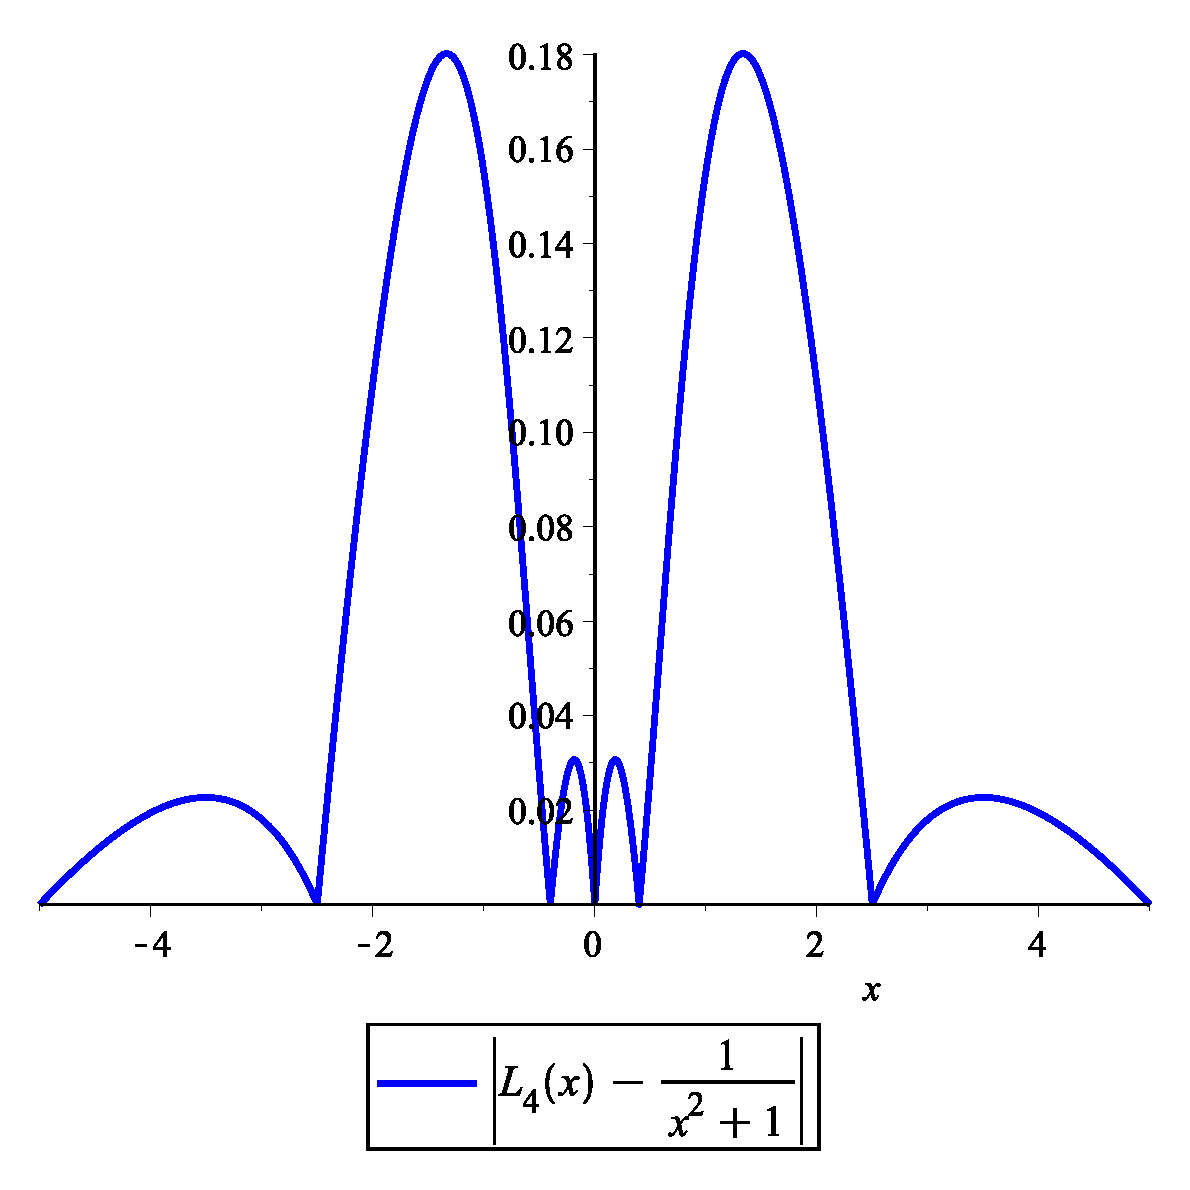
\includegraphics[width=0.25\textwidth]{err_L4.eps}
    \end{minipage}\\
    \begin{minipage}{0.65\textwidth}
      \scriptsize
      \begin{block}{}
        \texttt{\color{blue}
          \textbackslash usepackage\{graphicx\}\\
          \textbackslash begin\{document\}\\
          \textbackslash includegraphics[height=0.75\textbackslash textheight]\{imagen.png\}\\
          \textbackslash end\{document\}
        }\end{block} 
      \end{minipage} &
        \begin{minipage}{0.5\textwidth}
          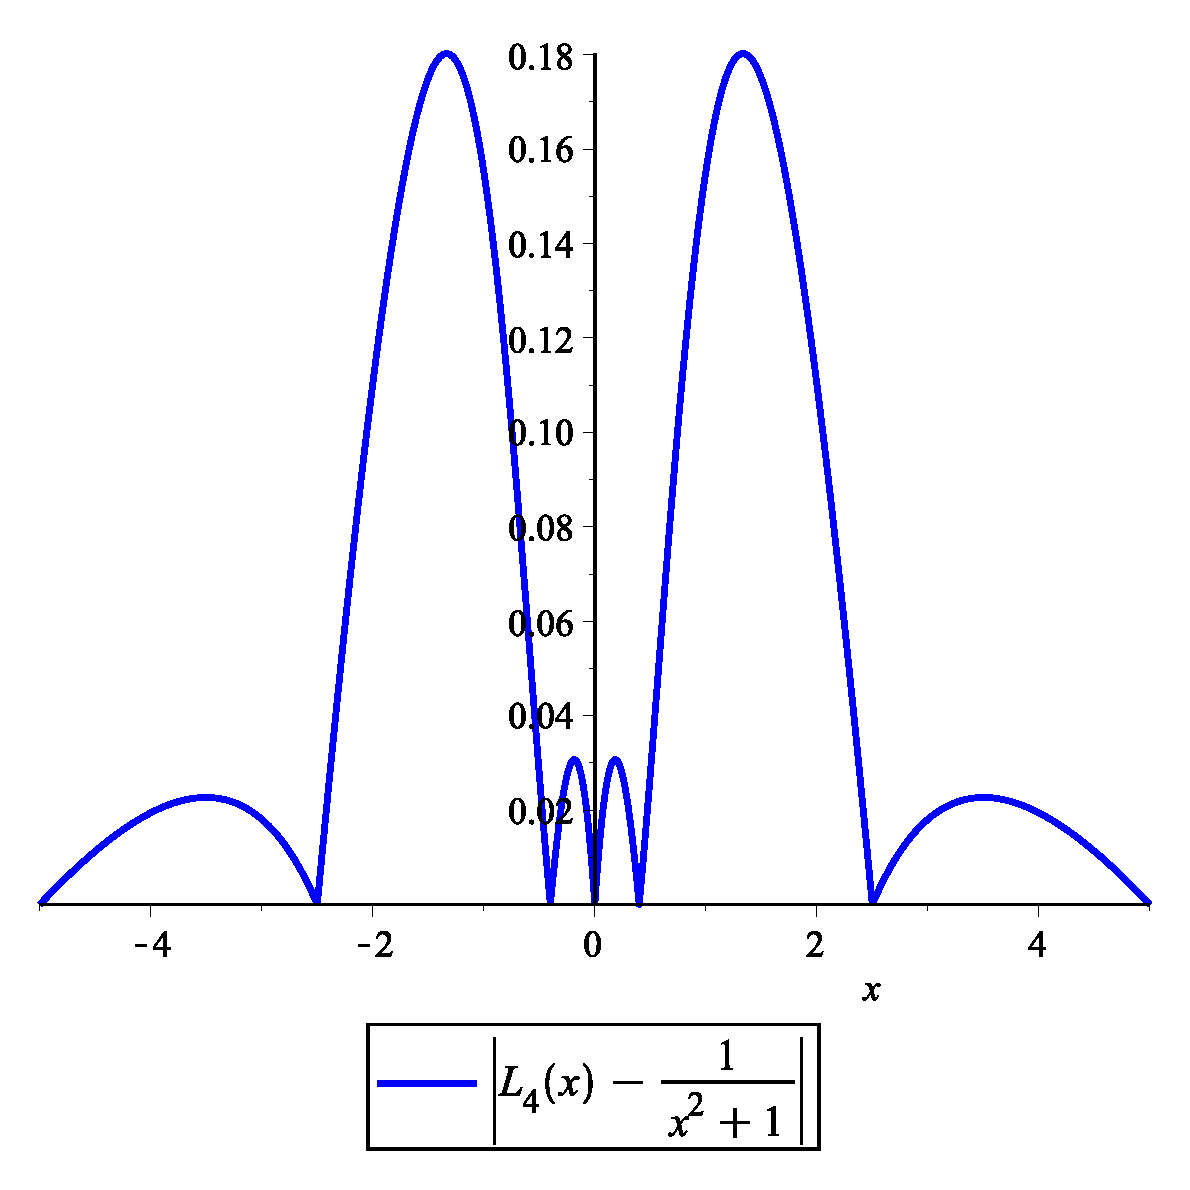
\includegraphics[height=0.7\textwidth]{err_L4.eps}
        \end{minipage}      
  \end{tabular}
\end{frame}
%%%%%%
\begin{frame}{Cambiando la apariecia de la imagen}
  \begin{itemize}
    \item También se puede cambiar la escala \texttt{\color{blue}scale} de las imágenes o hacerlas rotar de un ángulo dado con \texttt{\color{blue}angle}.
    \item<2-> La otra cosa que puede hacer es recortar una imagen con \texttt{\color{blue}clip} y \texttt{\color{blue}trim}.    
  \end{itemize}
  \uncover<3->{
  \begin{tabular}{ll}
    \scriptsize
    \begin{minipage}{0.5\textwidth}
      \begin{block}{}
        \texttt{\color{blue}
          \textbackslash usepackage\{graphicx\}\\
          \textbackslash begin\{document\}\\
          \textbackslash includegraphics[scale=0.15]\{imagen.png\}\\
          \textbackslash end\{document\}
        }
      \end{block}
    \end{minipage} &
    \begin{minipage}{0.3\textwidth}
      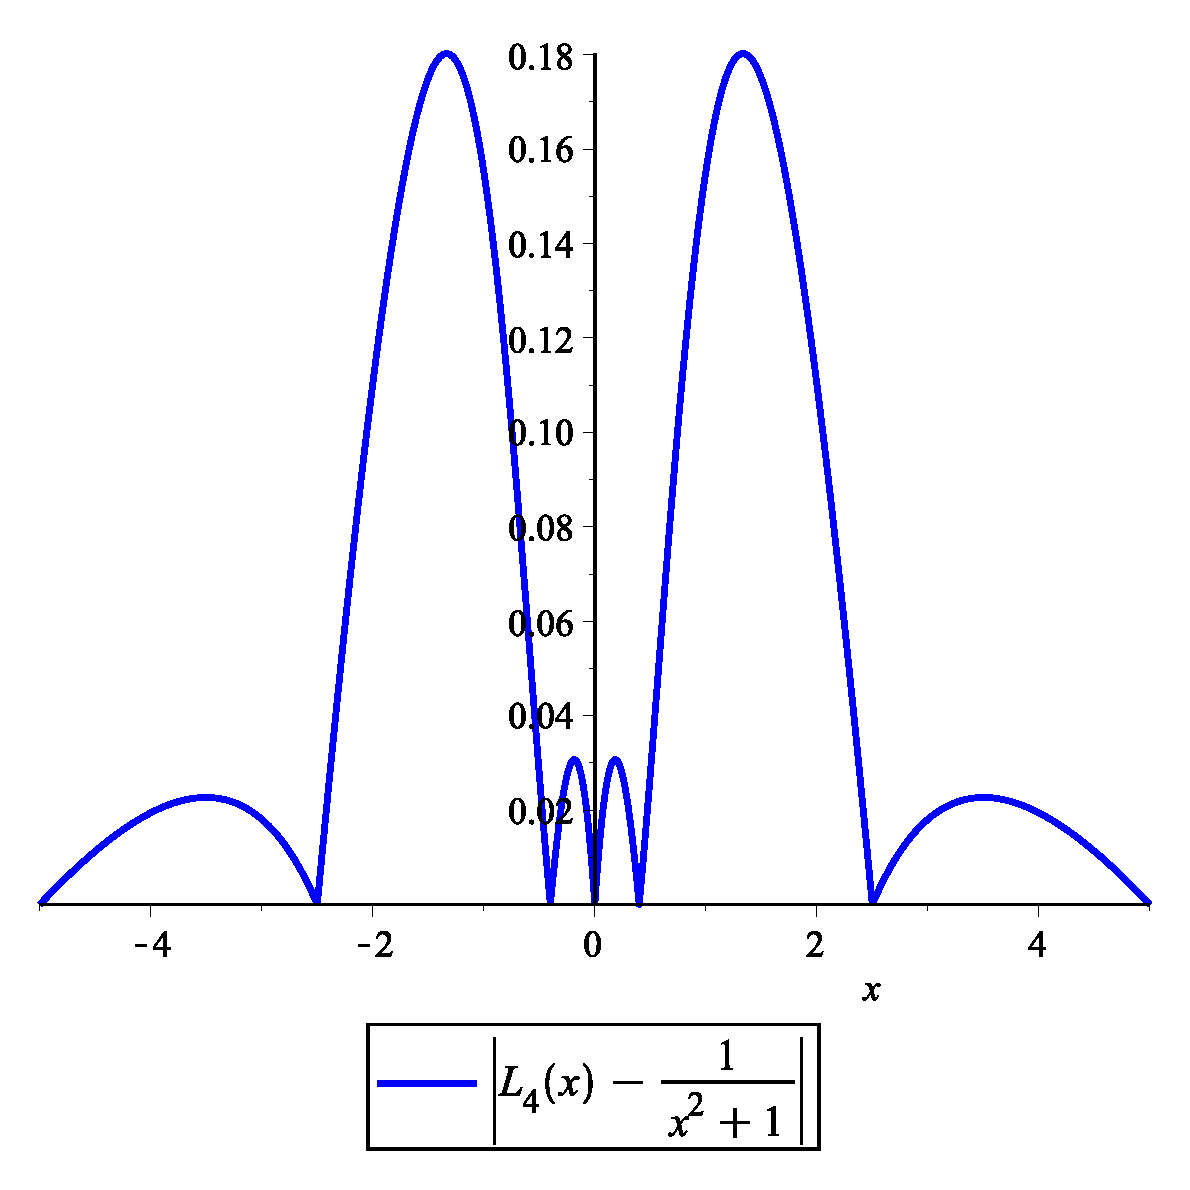
\includegraphics[scale=0.15]{err_L4.eps}
    \end{minipage}\\
    \begin{minipage}{0.5\textwidth}
      \scriptsize
      \begin{block}{}
        \texttt{\color{blue}
          \textbackslash usepackage\{graphicx\}\\
          \textbackslash begin\{document\}\\
          \textbackslash includegraphics[angle=45]\{imagen.png\}\\
          \textbackslash end\{document\}
        }
      \end{block}
    \end{minipage} &
    \begin{minipage}{0.3\textwidth}
      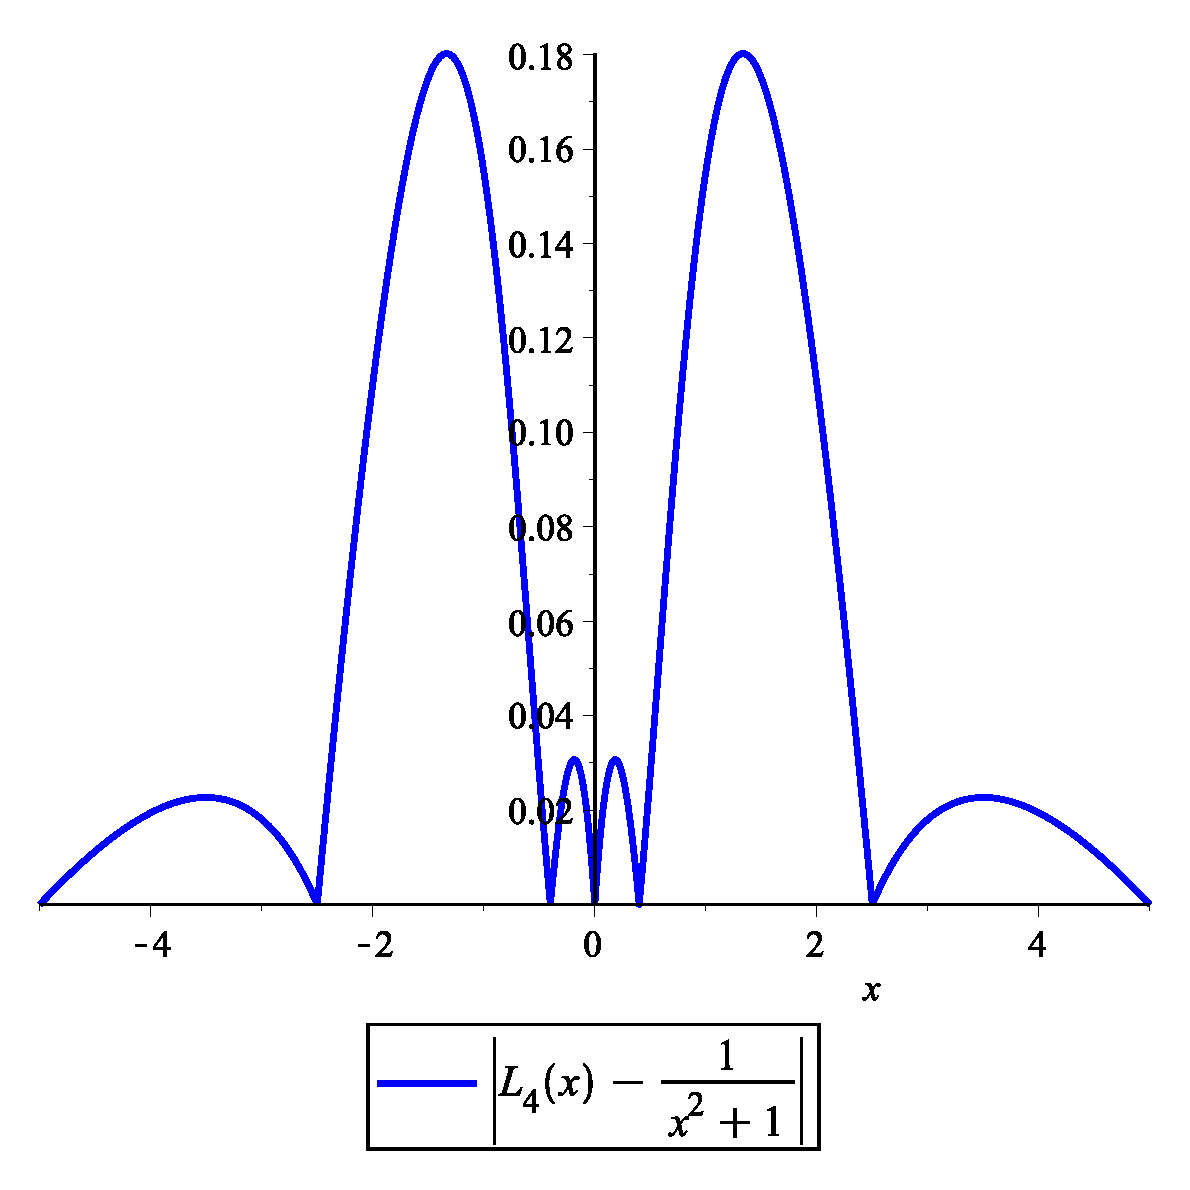
\includegraphics[scale=0.1,angle=45]{err_L4.eps}
    \end{minipage}
  \end{tabular}}
\end{frame}
%%%%%%
\begin{frame}{Cambiando la apariecia de la imagen}
  \begin{itemize}
    \item<1-> La otra cosa que puede hacer es recortar una imagen con \texttt{\color{blue}clip} y \texttt{\color{blue}trim}.    
  \end{itemize}
  \uncover<2->{
  \begin{tabular}{ll}
    \scriptsize
    \begin{minipage}{0.5\textwidth}
      \begin{block}{}
        \texttt{\color{blue}
          \textbackslash usepackage\{graphicx\}\\
          \textbackslash begin\{document\}\\
          \textbackslash includegraphics[clip,trim=100 50 50 400]\{imagen.png\}\\
          \textbackslash end\{document\}        
        }
      \end{block}
    \end{minipage} &
     \begin{minipage}{0.3\textwidth}
       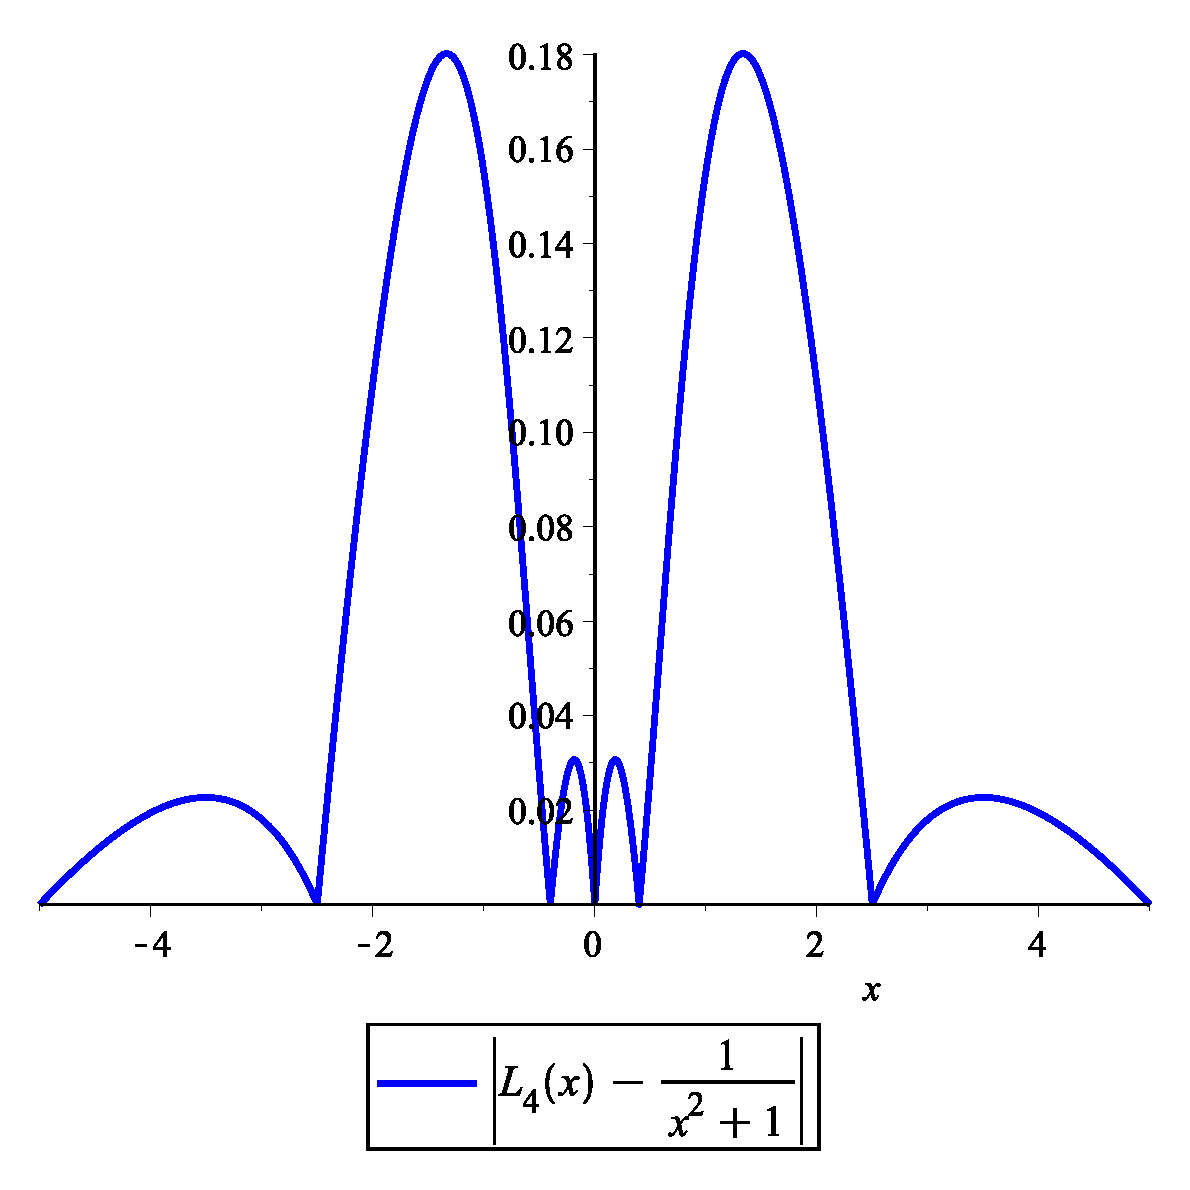
\includegraphics[clip,trim=100 50 50 400,scale=0.25]{err_L4.eps}
     \end{minipage}\\
     \begin{minipage}{0.5\textwidth}
       \scriptsize
       \begin{block}{}
         \texttt{\color{blue}
           \textbackslash usepackage\{graphicx\}\\
           \textbackslash begin\{document\}\\
           \textbackslash includegraphics[trim=0cm 0cm 0cm 0cm]\{imagen.png\}\\
           \textbackslash end\{document\}
         }
       \end{block}
     \end{minipage} &
     \begin{minipage}{0.3\textwidth}
       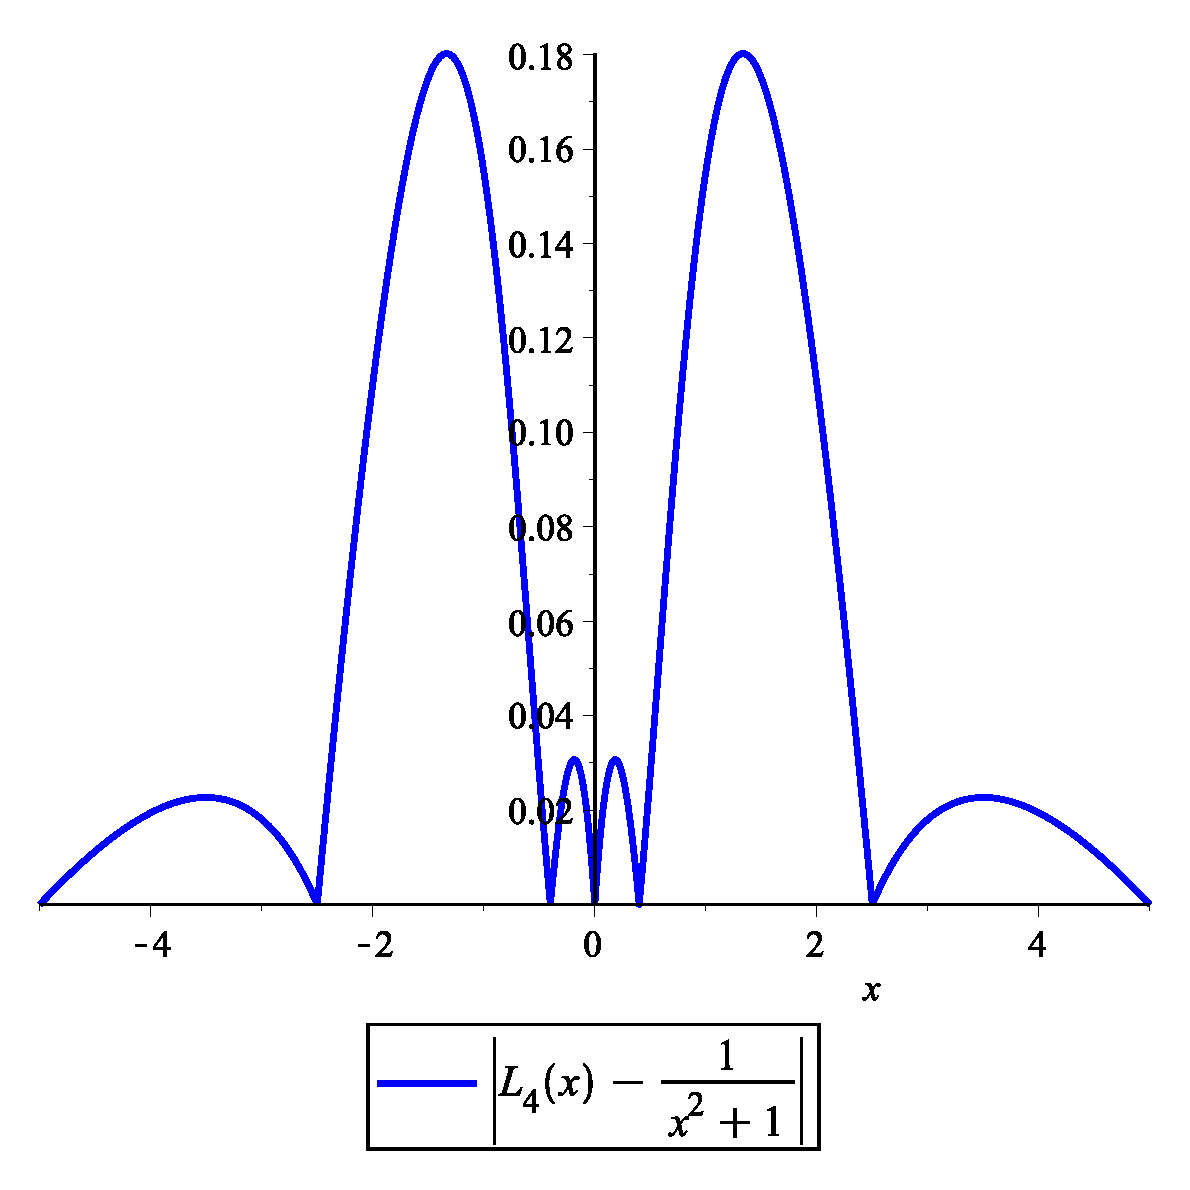
\includegraphics[trim=50 50 50 -40,scale=0.25]{err_L4.eps}
     \end{minipage}
  \end{tabular}}
\end{frame}
%%%%%%
\begin{frame}{Insertando Tablas}
  \begin{itemize}
    \item<1-> El paquete \texttt{\color{blue}array} añade más funcionalidades a las dadas por \LaTeX{} y que no forma parte del núcleo de \LaTeX{}.
    \item<2-> Para insertar tablas en \LaTeX, se usa el comando \texttt{\color{blue}tabular}.
    \item<3-> El comando \texttt{\color{blue}tabular} toma un argumento obligatorio, que es el alineamiento de las columnas.
  \end{itemize}
  \uncover<4->{  
  \begin{center}
    \scriptsize
    \begin{tabular}{|l|p{0.6\textwidth}|} % Using p for the description column
      \hline
      \textbf{Tipo} & \textbf{Descripción} \\ \hline
      l & columna justificada a la izquierda \\ \hline
      c & columna centrada \\ \hline
      r & columna justificada a la derecha \\ \hline
      p\{width\} & columna con un ancho \texttt{width} fijo; el texto sera automáticamente ajustado a la línea y justificado \\ \hline
      m\{width\} & como \texttt{p}, pero centrado verticalmente con respecto al resto del texto de la misma fila \\ \hline
      b\{width\} & como \texttt{p}, pero ajustado verticalmente a la parte baja de la celda \\ \hline
      w\{align\}\{width\} & imprime el contenido con un ancho \texttt{width} fijo, sobreimprimiendo si el texto es muy largo. Puede elegir el justificado horizontal \texttt{align} usando \texttt{l}, \texttt{c}, or \texttt{r}. \\ \hline
      W\{align\}\{width\} & como \texttt{w}, pero dando lugar a un mensaje de alerta «overfull box warning» si el texto es demasiado grande. \\ \hline
    \end{tabular}
  \end{center}}
\end{frame}
%%%%%%
\begin{frame}{Insertando Tablas}
  \begin{itemize}
    \item<1-> Las columnas \texttt{\color{blue}c} y \texttt{\color{blue}l} y \texttt{\color{blue}r} tendrán la anchura de la celda más ancha.
    \item<2-> Cada columna debe ser declarada, con lo que si se quiere tres columnas centradas, se tendrá que usar \texttt{\color{blue}ccc} en el preámbulo de la tabla. Los espacios son ignorados, con lo que \texttt{\color{blue}c c c} tendrá el mismo efecto.
    \item <3-> En el cuerpo de la tabla, las columnas se separan usando el símbolo \texttt{\color{blue}\&} y una nueva fila comienza con los símbolos \texttt{\color{blue}\textbackslash\textbackslash}.
  \end{itemize}
\end{frame}
%%%%%%
\begin{frame}{Insertando Tablas}
  \begin{tabular}{ll}
    \begin{minipage}{0.5\textwidth}
      \begin{block}{}
        \texttt{\color{blue}
          \textbackslash usepackage\{array\}\\
          \textbackslash begin\{document\}\\
          \textbackslash begin\{tabular\}\{lll\}\\          
          Animal  \& Comida \& Tamaño \textbackslash\textbackslash\\
          perro   \& carne  \& mediano \textbackslash\textbackslash\\
          caballo \& heno   \& grande  \textbackslash\textbackslash\\
          rana    \& moscas \& pequeño \textbackslash\textbackslash\\
          \textbackslash end\{tabular\}\\
          \textbackslash end\{document\}
        }
      \end{block}
    \end{minipage} &
    \begin{minipage}{0.5\textwidth}
      \begin{tabular}{lll}
        Animal  & Comida & Tamaño \\
        perro   & carne  & mediano \\
        caballo & heno   & grande \\
        rana    & moscas & pequeño \\
      \end{tabular}
    \end{minipage}
    \end{tabular}
\end{frame}
%%%%%%
\begin{frame}{Insertando Tablas}
  \begin{itemize}
    \item<1-> Si la columna de una tabla contine mucho texto, se tendrá problemas al colocarlo únicamente con \texttt{\color{blue}l},  \texttt{\color{blue}r} o \texttt{\color{blue}c}.
  \end{itemize}
  \uncover<2->{  
  \begin{center}
    \scriptsize
    \begin{tabular}{ll} 
    \begin{minipage}{0.5\textwidth}
      \begin{block}{}
        \texttt{\color{blue}
          \textbackslash usepackage\{array\}\\
          \textbackslash begin\{document\}\\
          \textbackslash begin\{tabular\}\{cl\}\\          
          Animal  \& Descripción \textbackslash\textbackslash\\
          perro   \& El perro es un miembro del género Canis, el cual forma parte 
          de los cánidos derivados del lobo y es uno de los carnívoros terrestres 
      más abundantes. \textbackslash\textbackslash\\
          gato \& El gato es una especie doméstica de pequeños mamíferos carnívoros. Es la única especie domesticada de la familia de los félidos y es a menudo llamado gato doméstico, para diferenciarlo de los miembros salvajes de la familia. \textbackslash\textbackslash\\
          \textbackslash end\{tabular\}\\
          \textbackslash end\{document\}
        }
      \end{block}
    \end{minipage} &
    \begin{minipage}{0.5\textwidth}
      \begin{tabular}{cl}
        Animal & Descripción \\
        perro  & El perro es un miembro del género Canis, el cual forma parte 
                de los cánidos derivados del lobo y es uno de los carnívoros terrestres 
            más abundantes. \\
        gato   & El gato es una especie doméstica de pequeños mamíferos carnívoros. Es la única especie domesticada de la familia de los félidos y es a menudo llamado gato doméstico, para diferenciarlo de los miembros salvajes de la familia. \\
      \end{tabular}
    \end{minipage}
    \end{tabular}
  \end{center}}
\end{frame}
%%%%%%
\begin{frame}{Insertando Tablas}
  \begin{itemize}
    \item<1-> El problema, es que el tipo de columna escribe el contenido de la celda en una única fila con el ancho que le corresponde, aunque haya un borde de página de por medio.
    \item <2-> Para evitar este problema se puede usar la columna \texttt{\color{blue}p\{ancho\}} especificando el ancho como argumento.
    \item <3-> También se puede usar el comando \texttt{\color{blue}b\{ancho\}},\texttt{\color{blue}m\{ancho\}},\texttt{\color{blue}w\{ancho\}}.
  \end{itemize}
  
\end{frame}  
%%%%%%
\begin{frame}{Insertando Tablas}
    \begin{center}
      \scriptsize
      \begin{tabular}{ll} 
      \begin{minipage}{0.5\textwidth}
        \begin{block}{}
          \texttt{\color{blue}
            \textbackslash usepackage\{array\}\\
            \textbackslash begin\{document\}\\
            \textbackslash begin\{tabular\}\{cp\{4cm\}\}\\          
            Animal  \& Descripción \textbackslash\textbackslash\\
            perro   \& El perro es un miembro del género Canis, el cual forma parte 
            de los cánidos derivados del lobo y es uno de los carnívoros terrestres 
        más abundantes. \textbackslash\textbackslash\\
            gato \& El gato es una especie doméstica de pequeños mamíferos carnívoros. Es la única especie domesticada de la familia de los félidos y es a menudo llamado gato doméstico, para diferenciarlo de los miembros salvajes de la familia. \textbackslash\textbackslash\\
            \textbackslash end\{tabular\}\\
            \textbackslash end\{document\}
          }
        \end{block}
      \end{minipage} &
      \begin{minipage}{0.5\textwidth}
        \begin{tabular}{cp{4cm}}
          Animal & Descripción \\
          perro  & El perro es un miembro del género Canis, el cual forma parte 
                  de los cánidos derivados del lobo y es uno de los carnívoros terrestres 
              más abundantes. \\
          gato   & El gato es una especie doméstica de pequeños mamíferos carnívoros. Es la única especie domesticada de la familia de los félidos y es a menudo llamado gato doméstico, para diferenciarlo de los miembros salvajes de la familia. \\
        \end{tabular}
      \end{minipage}
      \end{tabular}
    \end{center}
\end{frame}
%%%%%%
\begin{frame}{Insertando Tablas}
  \begin{itemize}
    \item<1-> El entorno \texttt{\color{blue}tabular} proporciona flexibilidad adicional; por ejemplo, se puede insertar líneas divisorias entre cada columnam, para separar las columnas.
    \item <2-> Se puede usar el comando \texttt{\color{blue}hline} para insertar una línea horizontal.
    \item <3-> Se puede usar el comando \texttt{\color{blue}cline} para insertar una linea con un estilo diferente.
    \item <4-> La lineas verticales se definen en cada columna insertando una barra vertical \texttt{\color{blue}|}.
    \item <5-> El paquete \texttt{\color{blue}booktabs} proporciona otras opciones para personalizar las tablas. No es aconsejable su uso con lineas verticales.
  \end{itemize}  
\end{frame}
%%%%%%
\begin{frame}{Insertando Tablas}
  \begin{center}
       \begin{tabular}{ll} 
         \begin{minipage}{0.5\textwidth}
           \begin{block}{}
             \footnotesize
             \texttt{\color{blue}
             \textbackslash usepackage\{array\}
             \textbackslash usepackage\{booktabs\}
             \textbackslash begin\{document\}
             \textbackslash begin\{tabular\}\{|c|c|c|\}
             \textbackslash toprule[2pt]
              item 11 \& item 12 \& item 13 \textbackslash\textbackslash\textbackslash\textbackslash\textbackslash hline\\
              item 21 \& item 22 \& item 23 \textbackslash\textbackslash\textbackslash\textbackslash \textbackslash cline{1-2}\\
              item 31 \& item 32 \& item 33 \textbackslash\textbackslash\textbackslash cmidrule[2pt](r){2-3}\\
              item 41 \& item 42 \& item 43 \textbackslash\textbackslash
              \textbackslash bottomrule[2pt]\\
              \textbackslash end\{tabular\}
              \textbackslash end\{document\}}
           \end{block}
         \end{minipage} &
       \begin{minipage}{0.5\textwidth}
        \footnotesize
    \begin{tabular}{|c|c|c|}
      \toprule[2pt]
     item 11 & item 12 & item 13 \\\hline
     item 21 & item 22 & item 23 \\\cline{1-2}
     item 31 & item 32 & item 33 \\\cmidrule[2pt](r){2-3}
     item 41 & item 42 & item 43 \\
      \bottomrule[2pt]    
    \end{tabular}    
       \end{minipage} 
     \end{tabular}
  \end{center}
\end{frame}
%%%%%%
\begin{frame}{Entornos Flotantes}
\begin{itemize}
  \item<1->Determinados contenidos, como por ejemplo tablas o imágenes, son bloques indivisibles.
  \item<2->Cuando no hay espacio suficiente en la página, pasan a colocarse en la siguiente página, dejando en la página anterior un espacio vertical vacío poco estético.
  \item<3->La solución consiste en incluir estos contenidos en un entorno flotante, que se ubicará automáticamente sin dejar espacios vacíos.
  \item<4->Como estos contenidos pueden aparecer lejos de su posición en el código fuente, para que no estén descontextualizados suelen llevar asociada una leyenda.
  \item<5->Existen dos entornos flotantes, para figuras y tablas.
  \begin{itemize}
    \item <6-> \texttt{\color{blue}figure} para figuras.
    \item <7-> \texttt{\color{blue}table} para tablas.
  \end{itemize}
\end{itemize}
\end{frame}
%%%%%%
\begin{frame}{Entornos Flotantes - Figuras}
  \begin{itemize}
    \item El entorno flotante para figuras es \texttt{\color{blue}figure} tiene el siguiente esqueleto.
  \end{itemize}
  \begin{center}
    \begin{minipage}{0.9\textwidth}
      \footnotesize
      \texttt{\color{blue}
      \textbackslash begin\{figure\}[posición]\\
      Código de la imagen\\
      \textbackslash caption\{leyenda\}\\
      \textbackslash label\{etiqueta\}\\
      \textbackslash end\{figure\}}
    \end{minipage}
  \end{center}
  \begin{itemize}
    \item<2-> El argumento posición indica la preferencia de ubicación de la figura(\texttt{\color{blue}h} en el lugar en el que aparece en el código fuente, \texttt{\color{blue}t} arriba, \texttt{\color{blue}b} abajo), intentará ubicar la figura en esa posición salvo que no sea posible.
    \item<3-> El comando \texttt{\color{blue}label} asigna una etiqueta al entorno flotante para poder referenciarlo
    \item<4-> Por su parte, el comando \texttt{\color{blue}caption} crea la leyenda de la figura.
  \end{itemize}
\end{frame}
%%%%%%
\begin{frame}{Entornos Flotantes - Tablas}
  \begin{itemize}
    \item El entorno flotante para tablas es \texttt{\color{blue}table} tiene el siguiente esqueleto.
  \end{itemize}
  \begin{center}
    \begin{minipage}{0.9\textwidth}
      \footnotesize
      \texttt{\color{blue}
      \textbackslash begin\{table\}[posición]\\
      Código de la tabla\\
      \textbackslash caption\{leyenda\}\\
      \textbackslash label\{etiqueta\}\\
      \textbackslash end\{table\}}
    \end{minipage}
  \end{center}
  \begin{itemize}
    \item<2-> Las tablas, al igual que las figuras, se enumeran automáticamente
    \item<3-> y pueden referenciarse después asignándoles una etiqueta con el comando \texttt{\color{blue}label}.
    \item <4-> Por su parte, el comando \texttt{\color{blue}caption} crea la leyenda de la tabla.
  \end{itemize}
\end{frame}  
\end{document}